%% Supplementary material -- same class and macros as main.tex
\documentclass[pdflatex,sn-mathphys-num]{sn-jnl}
\usepackage{graphicx,amsmath,amssymb,amsthm,booktabs,array,xcolor,xr}
\externaldocument[M-]{main}
\theoremstyle{thmstyleone}\newtheorem{theorem}{Theorem}
\newcommand{\Ts}{T_{\mathrm{s}}}
\newcommand{\cd}{c_{\mathrm{d}}}
\newcommand{\sd}{s_{\mathrm{d}}}
\newcommand{\gh}{\hat g}
\newcommand{\Hh}{\hat H}
\newcommand{\Op}[2]{{}^{\mathrm{#1}}\!\Delta^{#2}}
\newcommand{\eps}{\varepsilon}
\renewcommand{\thesection}{S\arabic{section}}
\renewcommand{\thetable}{S\arabic{table}}
\renewcommand{\thefigure}{S\arabic{figure}}
\renewcommand{\theequation}{S\arabic{equation}}
\raggedbottom
\begin{document}
\title[Supplementary material]{Supplementary Material for ``Definition-Consistent Variable-Order Fractional Operators from Fixed-Pole Banks: Structure, Error Guarantees, and Order Tracking''}
\author{\fnm{First} \sur{Author}}
\affil{\orgname{Institution}}
\abstract{This supplement collects secondary numerical results and implementation details. Section and equation numbers without the prefix S refer to the main paper.}
\maketitle

\section{Continuous-time switching results}\label{sup:ct}
Table~\ref{tab:e1} gives the numbers behind Fig.~\ref{M-fig:definition} of the main paper (Sect.~\ref{M-sec:res-def}).

\begin{table}[t]
\caption{Continuous time, step input: relative RMS error after a single switch. FP-out and FP-in are the fixed-pole bank with output and input schedule; Ou-par and Ou-cas are the hot-swapped Oustaloup forms. Arrows show $S=15\to41$; the cascade column is at $S=41$}\label{tab:e1}
\footnotesize\setlength{\tabcolsep}{4pt}
\begin{tabular}{@{}lccccc@{}}
\toprule
$\alpha_1\to\alpha_2$ & A--B gap & FP-out vs A & FP-in vs B & Ou-par vs A & Ou-cas, A / B\\
\midrule
$-0.3\to-0.7$ & 0.52 & $1.0\mathrm{e}{-4}\to1.7\mathrm{e}{-4}$ & $1.0\mathrm{e}{-4}\to5.1\mathrm{e}{-5}$ & $0.12\to0.042$ & 0.16 / 0.33\\
$+0.3\to+0.7$ & 0.65 & $2.1\mathrm{e}{-3}\to1.5\mathrm{e}{-5}$ & $4.2\mathrm{e}{-3}\to1.5\mathrm{e}{-4}$ & $0.14\to0.053$ & 1.6 / 1.7\\
$-0.5\to+0.5$ & 0.81 & $1.1\mathrm{e}{-3}\to4.3\mathrm{e}{-5}$ & $5.1\mathrm{e}{-4}\to3.1\mathrm{e}{-5}$ & $0.23\to0.085$ & 4.6 / 1.6\\
$+0.5\to-0.5$ & 1.35 & $9.8\mathrm{e}{-5}\to3.4\mathrm{e}{-5}$ & $9.4\mathrm{e}{-4}\to8.0\mathrm{e}{-6}$ & $0.25\to0.080$ & 0.24 / 0.87\\
\botrule
\end{tabular}
\footnotetext{On the fixed band $[10^{-3},10^{5}]$\,rad/s used here, the fixed-pole bank reaches its tail floor near $S=15$. The rule of Sect.~\ref{M-sec:design} chooses the band from the tolerance instead.}
\end{table}


\section{State maps for moving-pole realizations}\label{sup:maps}
This section expands Sect.~\ref{M-sec:res-maps} of the main paper.

\paragraph{Setup.} For six single switches (at sample 2000, window 2000), we fitted $\Phi$ by truncated least squares on a mixed training ensemble of 4 classes with 200 inputs each (white, piecewise-constant, multisine, Brownian). We tested on fresh ensembles of 150 inputs per class and on a unit step, sweeping the truncation threshold. Besides the most accurate map, we report a robust \emph{minimum-norm} map: the map of smallest norm whose validation error is within twice the best. The maps were then rounded to float32 and to 24-bit fixed point.

\paragraph{Results.} Figure~\ref{fig:maps} and Table~\ref{tab:e2} report the worst case over the switches and the input classes. In float64 the error falls from $0.14$ (parallel, hot swap) and $1.1\times10^4$ (cascade, hot swap) to $1.7\times10^{-7}$ and $6.2\times10^{-7}$ at $S=31$. The map is, however, a dense $S\times S$ matrix, with norm between $10^3$ and $5\times10^4$ even for the minimum-norm choice. Rounded to 24 bits, the map loses 3.5 to 4.3 orders of magnitude of accuracy in the parallel form and 7.4 to 9.1 in the cascade form for $S\ge21$. In the cascade form the 24-bit error exceeds 1, and even float32 rounding raises it to $0.26$--$0.81$ for $S\ge15$.

With a smooth derivative order quantized to 41 levels (80 grid crossings, parallel form), a chain of maps reduced the step-input error from $4.1\times10^{-2}$ to $1.2\times10^{-4}$ ($S=15$). The fixed-pole bank needs no map, and its definitional error is exactly zero. For the $P=1024$ order levels of Sect.~\ref{M-sec:hw}, maps between neighbouring levels alone would need about 56\,Mbit of storage at $S=33$ and 25 bits per entry, against 0.78--1.08\,Mbit for the whole coefficient table of the bank.

\begin{figure}[t]
\centering
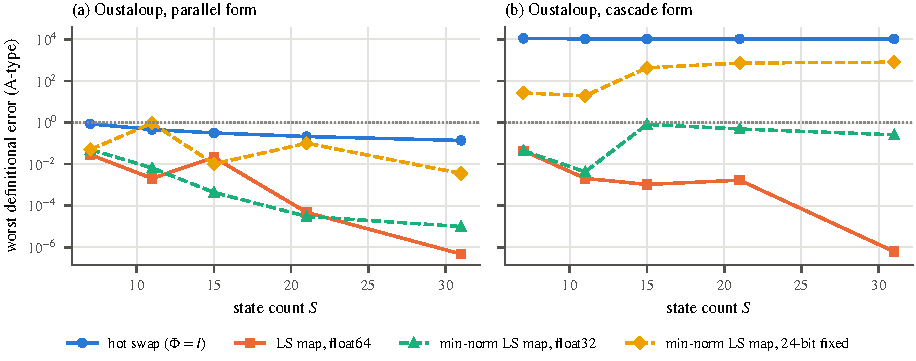
\includegraphics[width=\textwidth]{figs/fig_maps.pdf}
\caption{Worst definitional error (A-type) after one switch, over six switches and five input classes including the step. Hot swap versus least-squares state maps in float64, and the minimum-norm map rounded to float32 and to 24-bit fixed point. The dotted line marks an error of 1}\label{fig:maps}
\end{figure}

\begin{table}[t]
\caption{State maps for the Oustaloup forms: worst A-type definitional error over 6 switches and 5 input classes (including the step), and the largest norm of the minimum-norm map}\label{tab:e2}
\footnotesize\setlength{\tabcolsep}{4pt}
\begin{tabular}{@{}llccccc@{}}
\toprule
 & & & & \multicolumn{3}{c}{minimum-norm map}\\
\cmidrule(l){5-7}
$S$ & form & hot swap & LS, float64 & float64 ($\|\Phi\|_2$) & float32 & 24-bit\\
\midrule
7  & parallel & 0.86 & $2.8\mathrm{e}{-2}$ & $5.0\mathrm{e}{-2}$ ($3\mathrm{e}{4}$) & $5.0\mathrm{e}{-2}$ & $5.0\mathrm{e}{-2}$\\
15 & parallel & 0.32 & $2.1\mathrm{e}{-2}$ & $4.4\mathrm{e}{-4}$ ($5\mathrm{e}{4}$) & $4.3\mathrm{e}{-4}$ & $1.0\mathrm{e}{-2}$\\
31 & parallel & 0.14 & $4.7\mathrm{e}{-7}$ & $1.7\mathrm{e}{-7}$ ($5\mathrm{e}{3}$) & $9.8\mathrm{e}{-6}$ & $3.6\mathrm{e}{-3}$\\
7  & cascade & $1.1\mathrm{e}{4}$ & $4.4\mathrm{e}{-2}$ & $4.4\mathrm{e}{-2}$ ($9\mathrm{e}{2}$) & $4.4\mathrm{e}{-2}$ & $2.7\mathrm{e}{1}$\\
15 & cascade & $1.1\mathrm{e}{4}$ & $1.0\mathrm{e}{-3}$ & $3.2\mathrm{e}{-4}$ ($8\mathrm{e}{3}$) & $8.1\mathrm{e}{-1}$ & $4.3\mathrm{e}{2}$\\
31 & cascade & $1.1\mathrm{e}{4}$ & $6.2\mathrm{e}{-7}$ & $6.2\mathrm{e}{-7}$ ($4\mathrm{e}{4}$) & $2.6\mathrm{e}{-1}$ & $8.1\mathrm{e}{2}$\\
\botrule
\end{tabular}
\footnotetext{The fixed-point test rounds $\Phi$ to a single Q format; per-row scaling might do better. The fixed-pole bank needs $\Phi=I$ and has zero definitional error.}
\end{table}


\section{Which type does a hot swap implement?}\label{sup:hotswap}
Using the own-type references of Sect.~\ref{M-sec:results}, we asked which of the four types each hot-swapped realization is closest to, over 8 cases (four piecewise-constant order profiles, step and white-noise inputs) for $N=7$ and $N=15$:
\begin{itemize}
\item the fixed-pole bank is closest to A (output schedule) or B (input schedule) in all cases, at distances $\le2.1\times10^{-14}$;
\item the parallel Oustaloup form is closest to the A-type in all cases, at distances up to $0.42$;
\item for the cascade form with $\omega_h=10^3$\,rad/s, the closest type is A, B, D and E in two cases each, so the cascade has no consistent type; with $\omega_h=10^5$\,rad/s it is A or B, at distances up to $1.3\times10^{3}$;
\item with $\omega_h=10^5$\,rad/s, above the Nyquist frequency, the zero-order-hold members of the integral approximations have zeros outside the unit circle (moduli 3 to 41), and their own D- and E-types cannot even be formed in 6 of 8 cases.
\end{itemize}


\section{Fixed-point realization: details}\label{sup:hw}
This section expands Sect.~\ref{M-sec:hw} of the main paper. The design point is $R=4000$, $\eps=10^{-4}$ and $|\alpha|\le0.95$, giving $K=32$ plus the delay mode, and the orders come from a grid of $P=1024$ levels, $\alpha_i=0.95\,(2i/(P-1)-1)$.

\subsection*{Arithmetic in sample units}

The core runs in sample units ($\Ts=1$), where $\gh_0=1$ for every order. The inversion~\eqref{M-eq:inverse} then needs no divider: $v_n=x_n-\eta_n$. Physical units follow from one gain $\Ts^{-\alpha_n}$, applied at the output for the A- and E-types and at the input for the B- and D-types. This follows directly from~\eqref{M-eq:A}--\eqref{M-eq:E}; for the E-type, substitute $z_n=\Ts^{-\alpha_n}\zeta_n$.

The number formats are as follows:
\begin{itemize}
\item \emph{Signals:} $W_S$-bit two's complement with $F$ fractional bits.
\item \emph{States:} $W_{ST}=W_S+13$ bits. Each mode stores its state scaled by a power of two $2^{G_k}$ (one gain per schedule) so that its own bound uses the full word. Without this scaling, the input-scheduled slow modes lose their increments $c_kv_n$, which lie far below the signal LSB; the B- and E-type errors were then $2\times10^{-2}$ to $0.66$.
\item \emph{Coefficients:} a $W_M$-bit mantissa with a 7-bit shift.
\end{itemize}
Products are rounded as $\mathrm{mulsh}(a,M,S)=(aM+2^{S-1})\gg S$. Algorithm~\ref{M-alg:core} of the main paper gives one sample of the core in exact arithmetic; the bit-accurate golden model and the RTL use the same sequence with the formats above.



\subsection*{Dynamic range: two operating envelopes}

For $|x|\le1$ over $4000$ samples, the frozen-order $\ell_1$ bound on the output is $2696$. For the A-type this bound holds under any switching, because each output uses the weights of a single order; for the B-type the switching stress tests stayed within it. For the D- and E-types, switching from an integral to a derivative order drives the output to $2.2\times10^6$ under a DC input, 820 times the frozen-order bound. The new inverse acts on a history that has grown under the old order. This is the behaviour of the recursive definitions themselves, not an artefact of the bank. We therefore size two envelopes with a factor-two margin: 14 integer bits for the forward types only (A/B), and 24 integer bits for all four types (A/B/D/E).

\subsection*{Quantization and inverse stability}

Quantization can undo the DC floor. Coefficients and pole steps are dyadic rationals, so the signs of $\Hh_q(\pm1)$ of every quantized ROM row can be evaluated exactly in rational arithmetic, which we did. With the floating-point floor alone:
\begin{itemize}
\item in the A/B configuration, 64 of the 512 positive-order rows have $\Hh_q(1)\le0$, the worst having its dominant inverse pole at $1+4.8\times10^{-6}$ (e-folding time $2.1\times10^5$ samples);
\item in the A/B/D/E configuration, 51 of 512 rows have $\Hh_q(1)\le0$, the worst ($\alpha=0.855$) having its pole at $1+1.9\times10^{-9}$ (e-folding time $5.2\times10^{8}$ samples, about 9 minutes at 1\,MS/s).
\end{itemize}
$\Hh_q(-1)$ was positive in every row. The \emph{quantization-aware} DC floor raises the delay mantissa in LSB steps until $\Hh_q(1)$ is at least the floating-point value $\Hh(1)$. It brings both counts to zero without any measurable change in accuracy.

\subsection*{Word length}

We swept $W_S\in\{32,\dots,56\}$ and $W_M\in\{16,18,25,32\}$ (Fig.~\ref{fig:wordlength}). The test set comprised 3 order profiles (random piecewise, a new order every sample, a sign-changing switch), 3 inputs, and all types of the envelope. A configuration was accepted if, for every type, its error against the literal definition was at most the floating-point bank's error plus $0.1\eps$. The smallest accepted configurations were:
\begin{itemize}
\item A/B: $W_S/W_{ST}/W_M=36/49/16$;
\item A/B/D/E: $48/61/25$.
\end{itemize}
With an 18-bit mantissa the D- and E-types stall near $10^{-3}$, because the inversion is ill-conditioned: the low-frequency gain of a derivative bank is about $R^{-\alpha}$. The floating-point bank itself has D- and E-type output errors up to $6\times10^{-4}$ at this design point, although its weight error is $10^{-4}$. This is the cancellation effect of Corollary~\ref{M-cor:bound}, amplified by the inversion.

\begin{figure}[t]
\centering
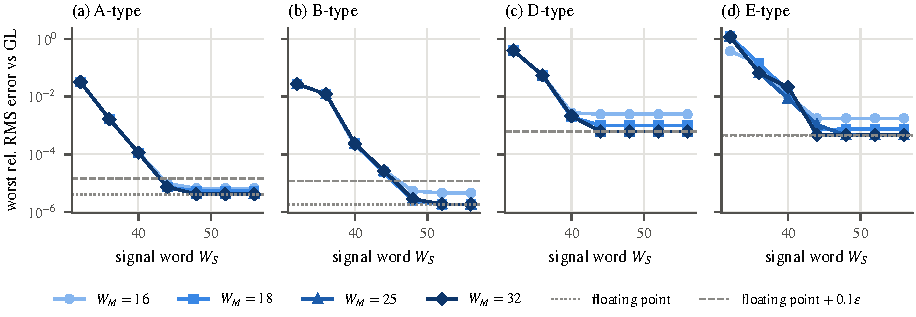
\includegraphics[width=\textwidth]{figs/fig_wordlength.pdf}
\caption{Word length, A/B/D/E envelope: worst relative RMS error against the literal definitions versus signal word $W_S$ (state word $W_S+13$), for four mantissa widths. Dotted: floating-point bank; dashed: acceptance limit}\label{fig:wordlength}
\end{figure}



\section{Streaming mBm: details}\label{sup:mbm}
This section expands Sect.~\ref{M-sec:mbm} of the main paper.

Further alternatives to mBm treat a varying Hurst exponent differently. The incremental mBm of \'Sl\c{e}zak and Metzler~\cite{slezak2023} is defined through the covariance of its increments and shares the property that a change of $H$ acts only on new increments. Other alternatives to mBm include:
\begin{itemize}
\item the multifractional processes of Surgailis, built by nonhomogeneous fractional integration of white noise~\cite{surgailis2008}, whose covariance is not a local function of $H(t)$ and $H(t')$ as it is for mBm~\cite{bardet2013};
\item the integrated fractional white noise of Sly, proposed to avoid the extreme changes in magnitude of mBm~\cite{sly2007}.
\end{itemize}
Conversely, the variable-Hurst fBm of Ryvkina uses the current Hurst value in its kernel and has discontinuous paths wherever $H$ jumps~\cite{ryvkina2015}, like the A-type. VO operators have been used to synthesize multifractional Gaussian noise before~\cite{sheng2011}, and simulation methods for mBm include~\cite{chan1998}. Exact methods for stationary Gaussian processes such as circulant embedding~\cite{wood1994} rely on stationarity and do not apply directly when $H$ varies.

\paragraph{Results.} Table~\ref{tab:mbm} and Fig.~\ref{M-fig:mbm} summarize the results. The bank was designed by the rule for $\eps=10^{-4}$ and $0.05\le H\le0.95$, giving $K=22$, 24 and 26 for $n=1024$, 4096 and 16\,384.

Second-order statistics were computed exactly, without Monte Carlo, from the $n\times n$ weight matrix of the generator. The variance agreed with the exact formula to $3.1\times10^{-5}$ and the covariance to $1.7\times10^{-6}$.

The local Hurst exponent was estimated by generalized quadratic variations~\cite{istas1997,coeurjolly2005}; see also~\cite{bardet2013}. For constant $H$ the estimator itself has a bias of $+0.06$ at $H=0.2$ and a standard deviation of $0.06$ (window 1024). For varying $H$ its mean followed $H(t)$ with RMSE $0.014$ to $0.036$, equally for both types.

The two types differ sharply at a jump of $H$ from $0.3$ to $0.8$. The A-type variance jumps from 119 to $1.5\times10^5$, and the path is discontinuous: the squared increment at the jump is $1.3\times10^5$ times the typical one. The B-type is continuous (ratio 1.0), in line with the behaviour reported for MMFBM and incremental mBm~\cite{wang2023mmfbm,slezak2023}. Which definition to use is therefore a modelling decision with visible consequences, as also argued in~\cite{wang2023mmfbm}. The bank makes either choice available at the same cost.

\begin{table}[t]
\caption{Streaming mBm with the fixed-pole bank}\label{tab:mbm}
\small
\begin{tabular}{@{}>{\raggedright\arraybackslash}p{0.44\textwidth}>{\raggedright\arraybackslash}p{0.52\textwidth}@{}}
\toprule
Quantity & Result\\
\midrule
integer split, correct order (A first, B last) & $\le9\times10^{-15}$\\
integer split, reversed order & $0.1$ to $1.3$\\
path vs literal GL, same noise & A $\le1.9\times10^{-6}$, B $\le2.4\times10^{-6}$\\
exact variance / covariance ($n=2048$) & $\le3.1\times10^{-5}$ / $\le1.7\times10^{-6}$ (Frobenius)\\
local Hurst tracking, varying $H$ (400 paths) & RMSE of mean 0.014 to 0.036, A and B alike\\
variance before/after a jump of $H$ from $0.3$ to $0.8$ & A $119\to1.5\times10^{5}$; B $119\to119$\\
cost per sample & bank 47 to 55 MACs ($n$-independent); direct GL $n/2$ on average\\
fixed-point core A/B (36/49/16), vs float & A $1.8\times10^{-5}$, B $8.9\times10^{-4}$\\
fixed-point core A/B/D/E (48/61/25), vs float & A $3.8\times10^{-6}$, B $1.2\times10^{-4}$\\
\botrule
\end{tabular}
\end{table}

\paragraph{Hardware.} The cores of Sect.~\ref{M-sec:hw} generate the same processes bit-exactly from integer noise. For the A-type, the accumulator sits in front of the core and is exact (an integer sum), so the small A/B core suffices. For the B-type, the accumulator follows the core and integrates its low-frequency rounding errors. The B-type therefore benefits from the wider configuration (Table~\ref{tab:mbm}, last two rows). Input scales were $2^{-9}$ for A and $0.25$ for B, chosen to keep the accumulated A-type input within the signal range.



\section{B-type step response}\label{sup:stepB}

The B-type operator in continuous time processes each input sample with the kernel of its entry order: $y(t)=\int_0^t K(t-\tau,\alpha(\tau))u(\tau)\,\mathrm d\tau$ with $K(s,a)=\partial_sF(s,a)=s^{-a-1}/\Gamma(-a)$, taken in the finite-part sense for $a>0$. For $u=1$, let $G(\tau)=F(t-\tau,\alpha(\tau))$. Then
\[
\frac{\mathrm dG}{\mathrm d\tau}=-\partial_sF(t-\tau,\alpha(\tau))+\partial_aF(t-\tau,\alpha(\tau))\,\dot\alpha(\tau),
\]
so $y(t)=G(0)-G(t)+\int_0^t\partial_aF\,\dot\alpha\,\mathrm d\tau$. The finite part removes $G(t)=F(0^+,\alpha(t))$, and $G(0)=F(t,\alpha(0))$. This gives~\eqref{M-eq:stepB}. For a piecewise-constant order, $\dot\alpha$ is a sum of Dirac impulses and the integral becomes the stated finite sum. In the experiments the smooth case was evaluated by adaptive quadrature after the substitution $s=v^m$ with $m(1-\alpha_{\max})\ge2$, which removes the weak singularity at $s=0$.

\section{Large-lag alias term}\label{sup:alias}

For large $r$ the integrand of~\eqref{M-eq:betax} is concentrated at $u=O(1/r)$, where $(1-e^{-u})^a\approx u^a$. Hence $f(x)\approx e^{(1+a)x}e^{-\rho e^x}$ with $\rho=r-a$. Its Fourier transform is $\hat f(\omega)=\Gamma(1+a-\mathrm i\omega)\rho^{-(1+a-\mathrm i\omega)}$, and $\hat f(0)=\Gamma(1+a)\rho^{-(1+a)}$ is the integral itself. The relative error of the infinite trapezoidal rule is $\sum_{k\neq0}\hat f(2\pi k/h)/\hat f(0)$, dominated by $k=\pm1$. Stirling's formula, $|\Gamma(1+a-\mathrm i\omega)|\sim\sqrt{2\pi}\,\omega^{a+1/2}e^{-\pi\omega/2}$, at $\omega=2\pi/h$ gives~\eqref{M-eq:Eq}. The result does not depend on $r$, which justifies the name large-lag term.

\bibliography{refs}
\end{document}
